% I'm not totally sure, if this should be described together or seperate, but somehow or SCRUM approach and the Redmine
% stuff should be mentioned somewhere before the developing part and as this are probably only three pages or somethin
% it probably could be integrated here
\chapter{Project Management and System Requirements}\label{chap:systemRequirements}

\section{Project Workflow}\label{sec:workflow}

To make it possible to work efficiently together in our distributed environment, the team uses 
\href{http://www.redmine.org/}{Redmine} as it's project management tool, which you can access under:

\begin{itemize}
\item \url{http://tickets.unplagged.com}
\end{itemize}

If you register there, an administrator should grant you access to the tickets and the wiki, so that you can participate
in solving the problems at hand. Our current workflow 

% Redmine description, Meetings, Debbie, Scrum Cards, Server, Website


\begin{figure}[!h]
    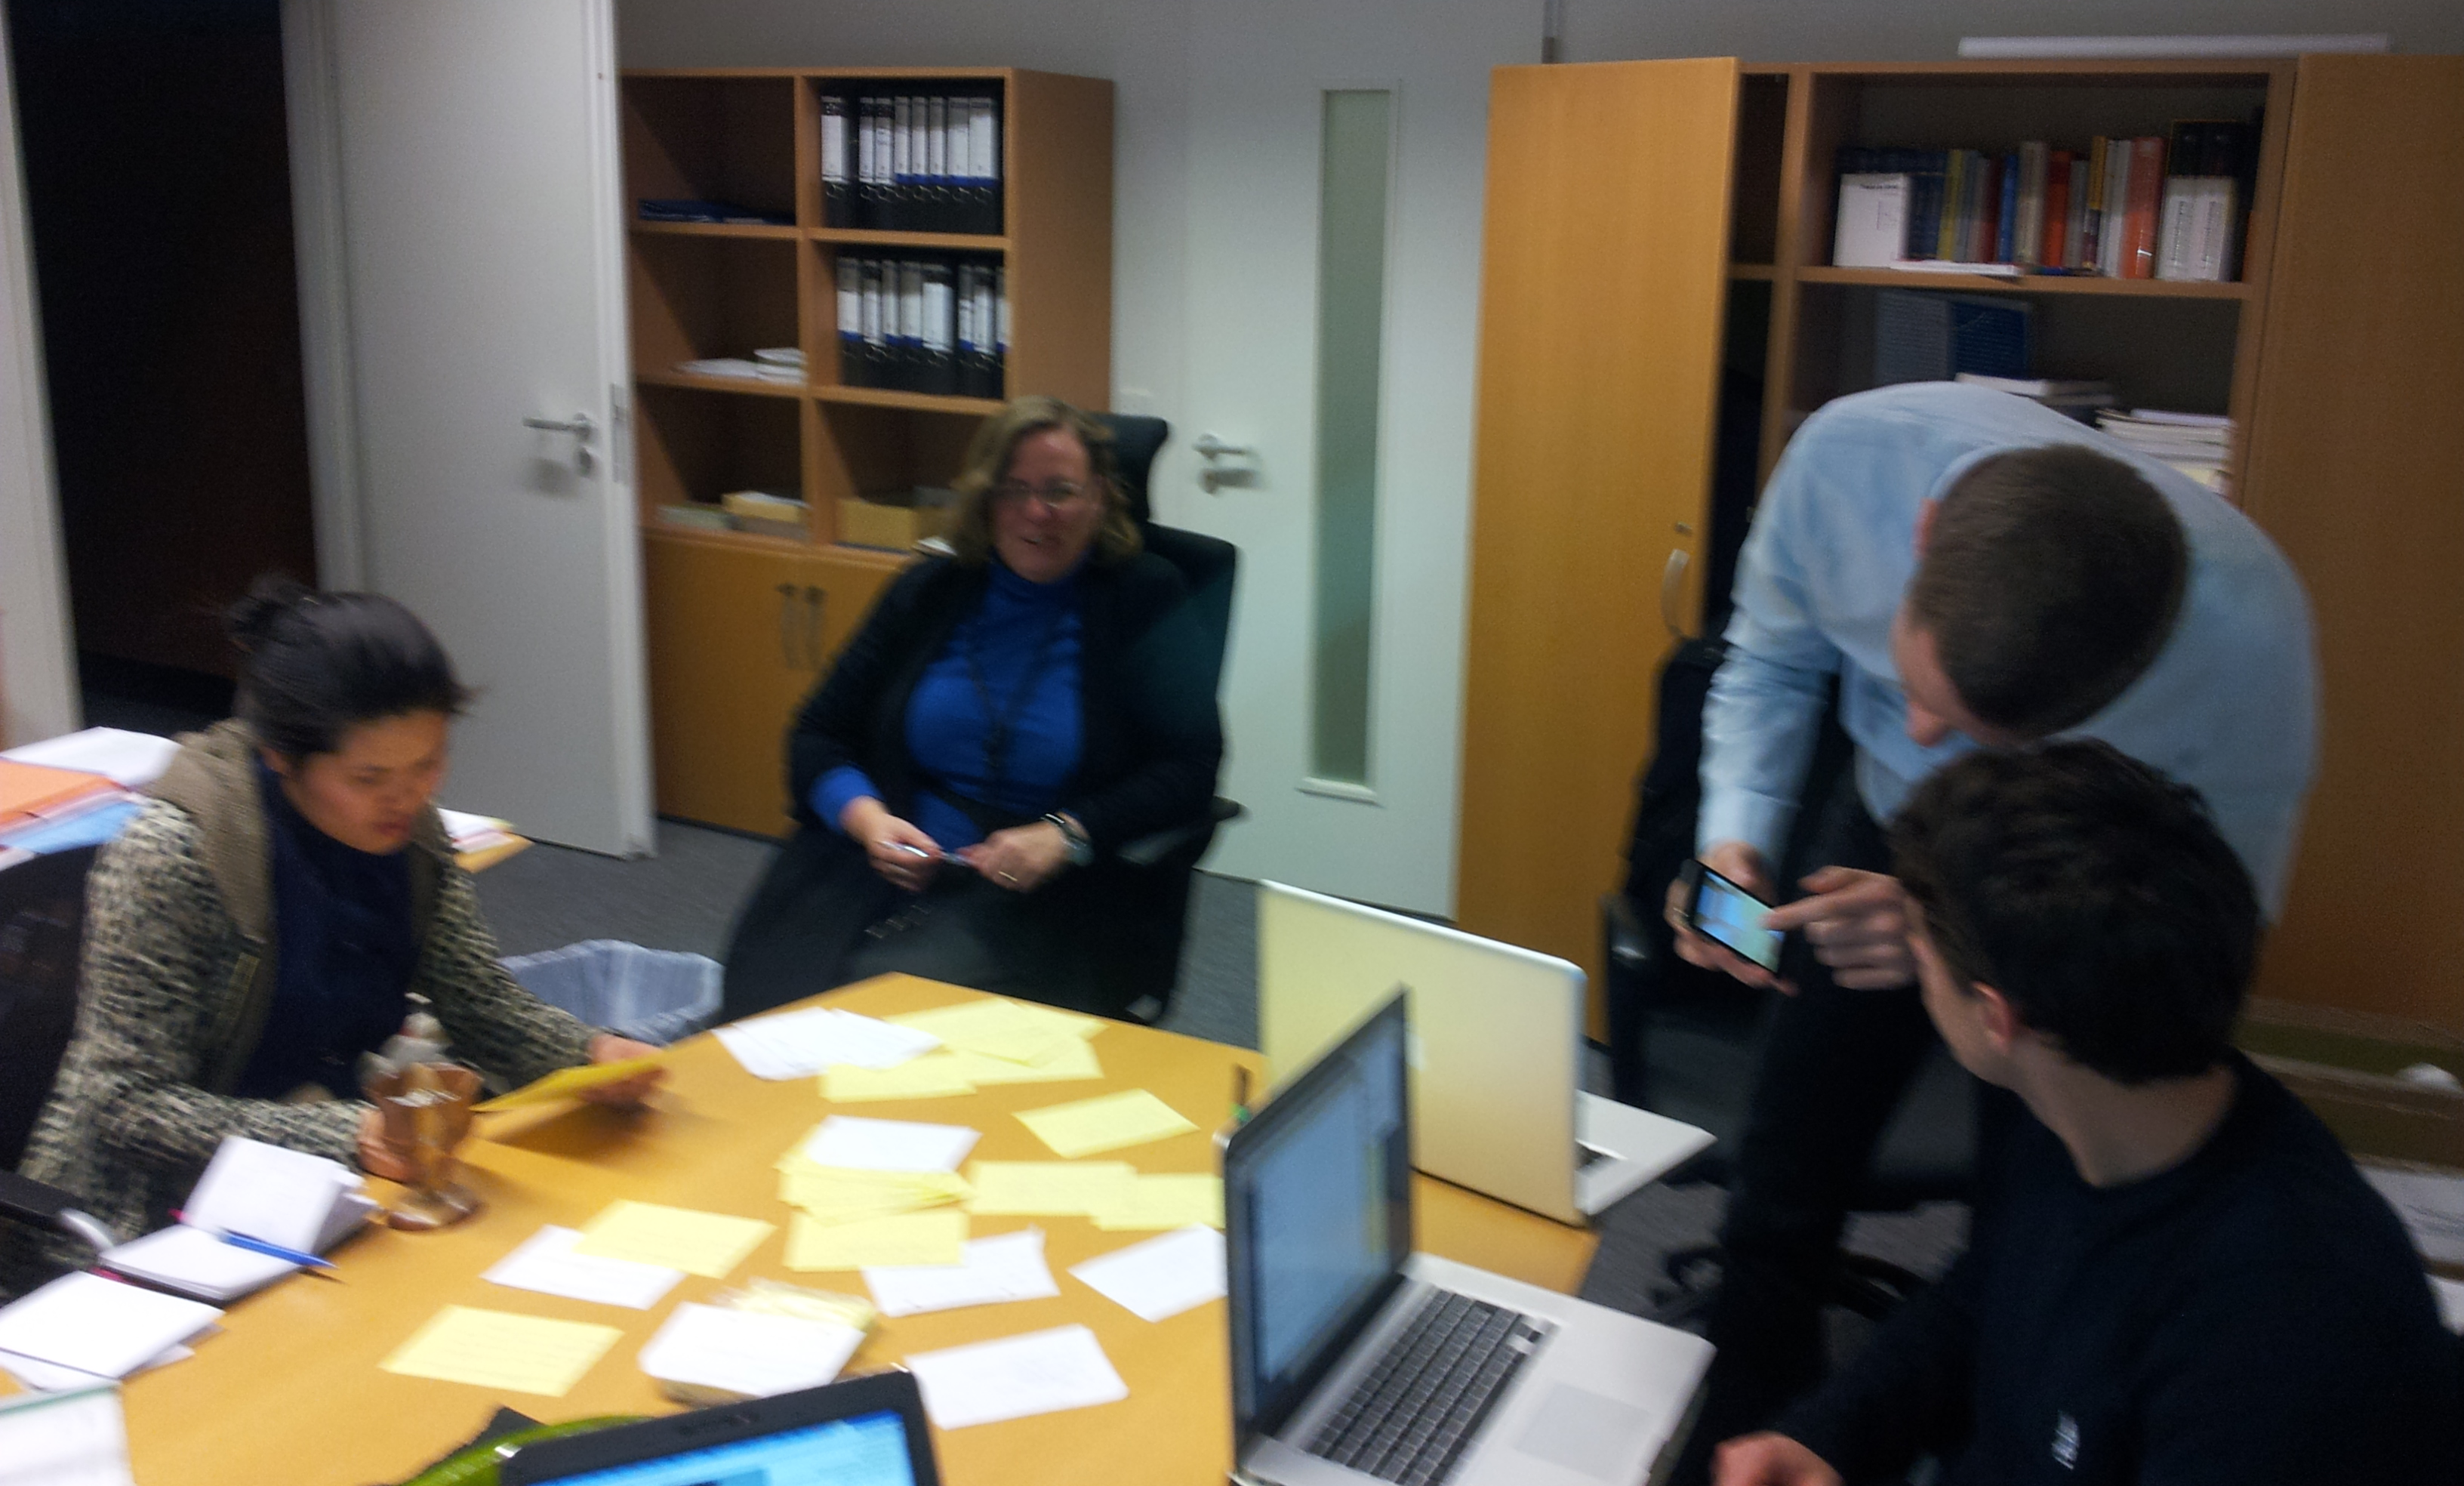
\includegraphics[width=0.8\textwidth]{images/2011-11-15-user-stories-6.jpg}
  \caption{Scrum Meeting}
  \label{fig:scrumming}
\end{figure}

\begin{figure}[!h]
    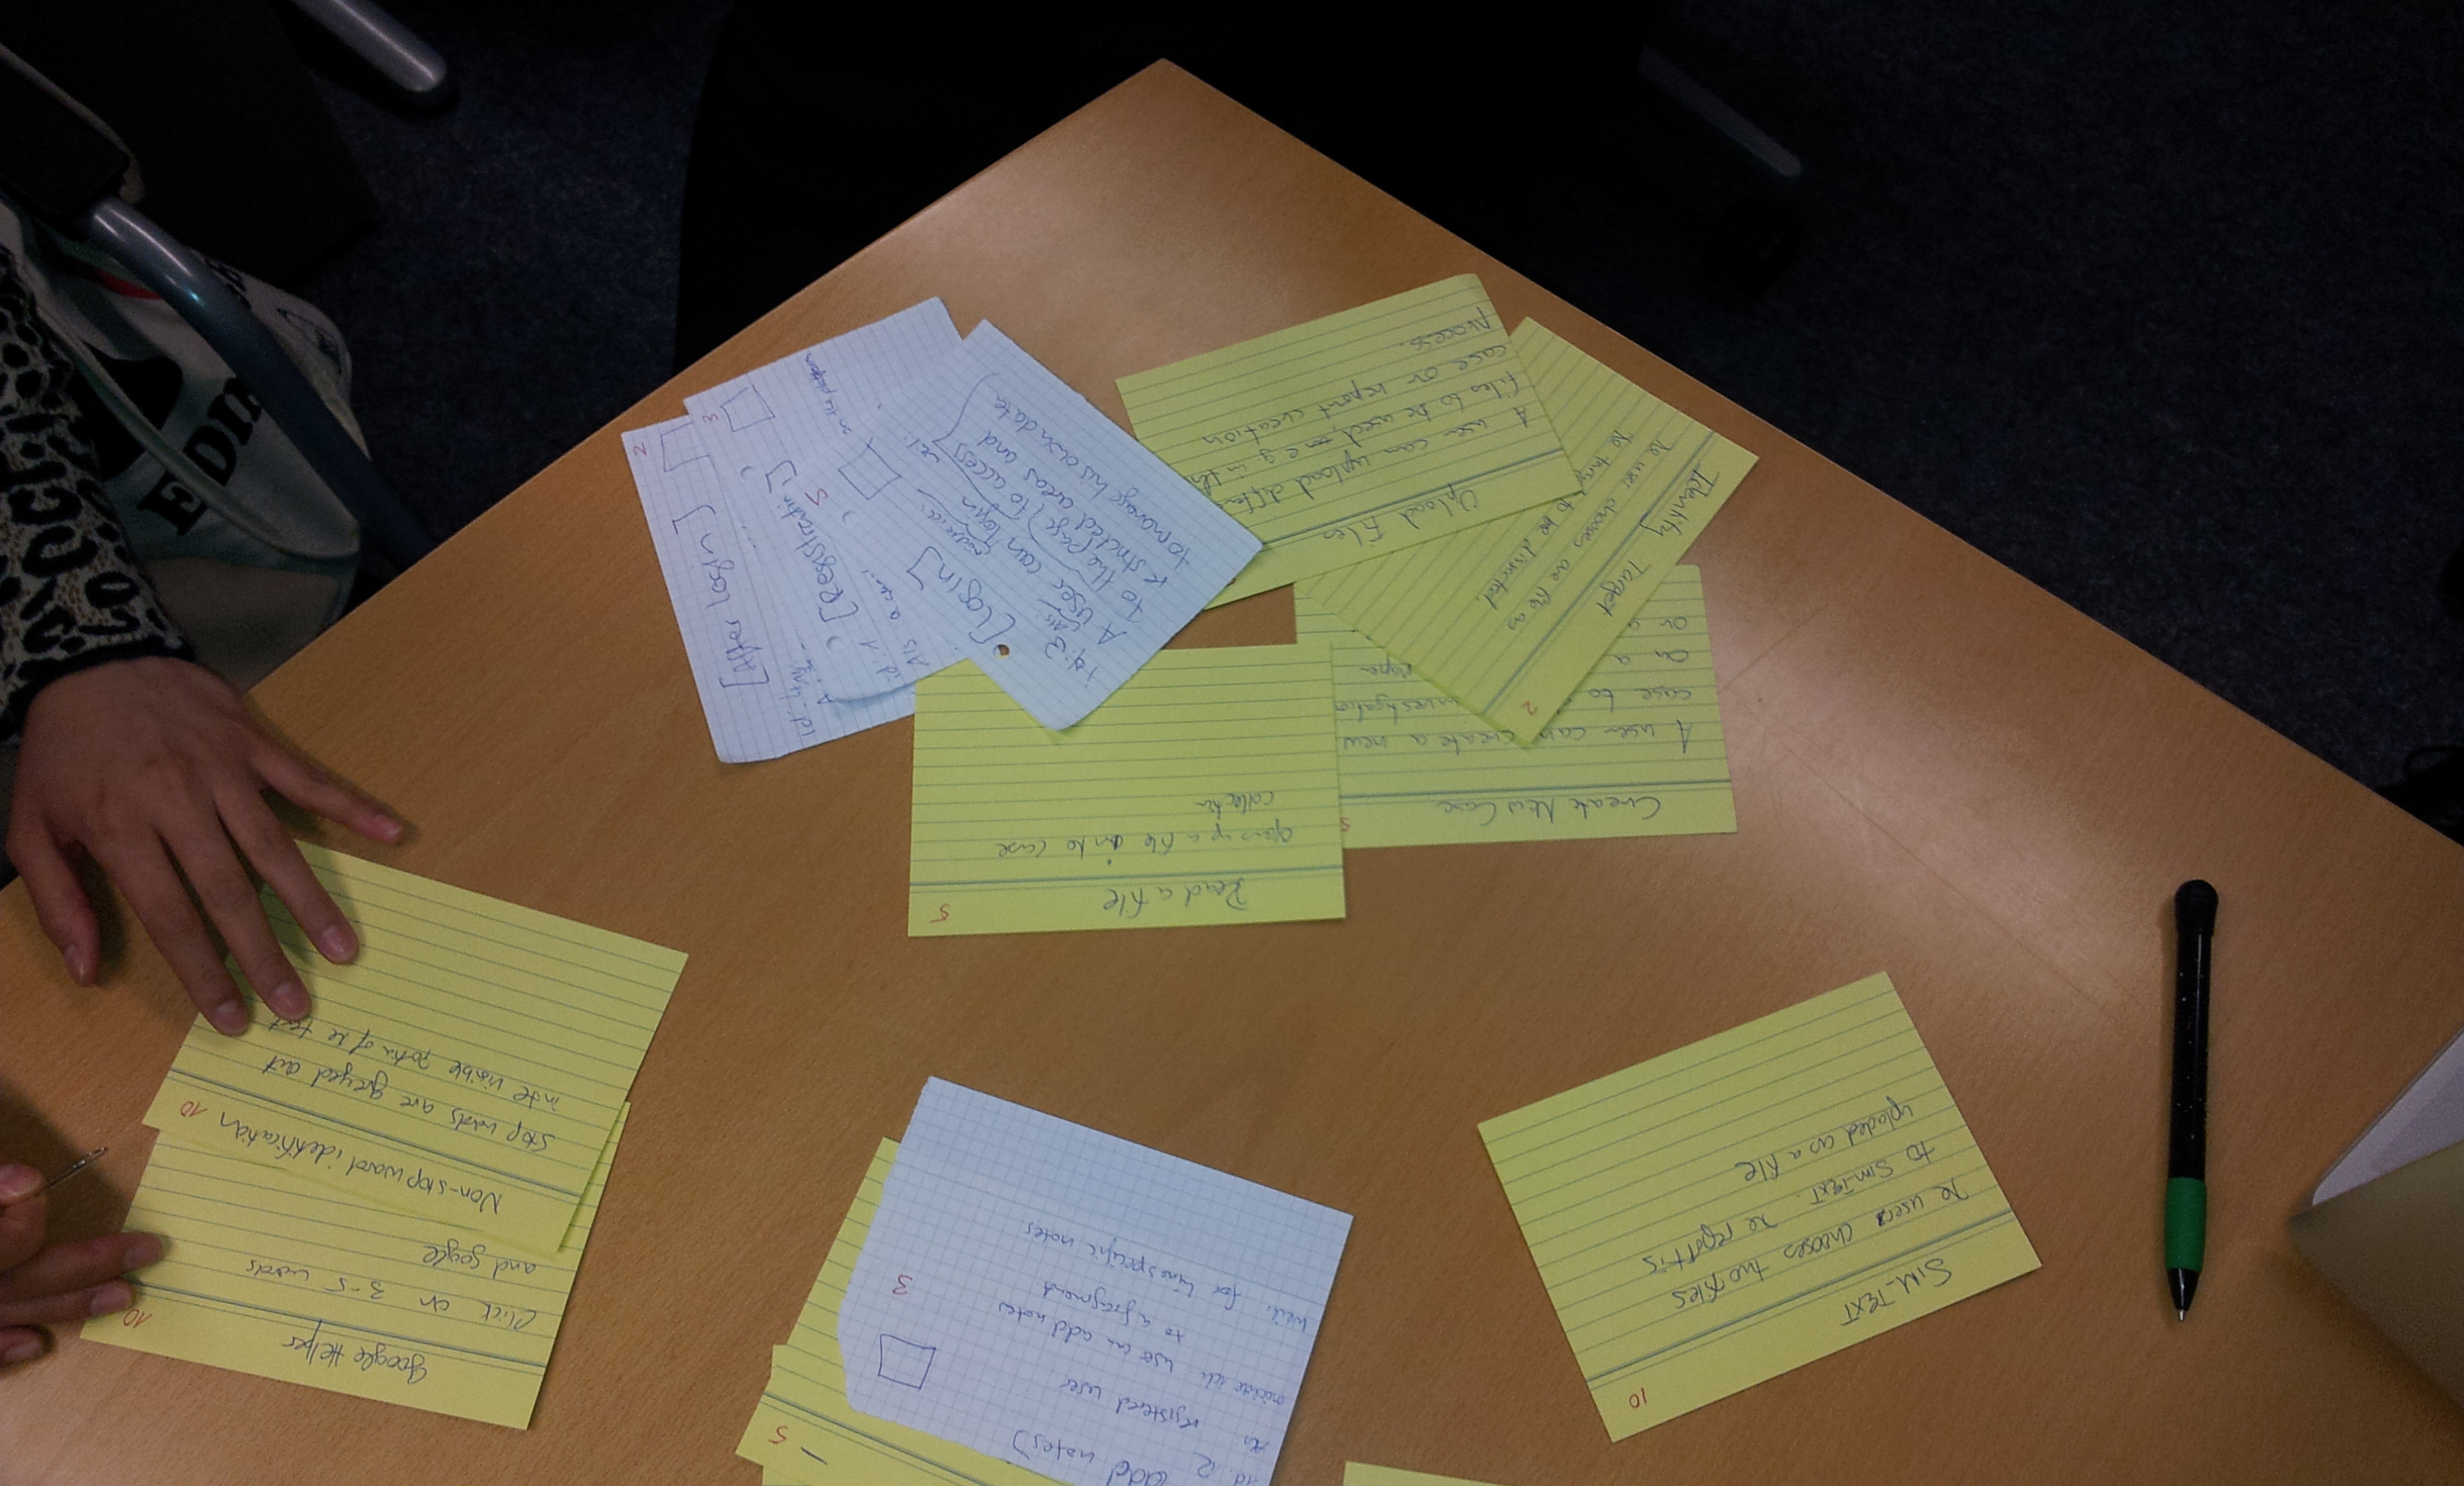
\includegraphics[width=0.8\textwidth]{images/2011-11-15-user-stories-4.jpg}
  \caption{User Stories}
  \label{fig:userStories}
\end{figure}

\section{Target Group}

\section{User roles}

\section{Basic functionalities}

\section{Document Parser}

\section{Detection Modes}

\section{Plugin Architecture}

%Perhaps better on the way for every part?
\section{Use Cases}
